\chapter{Rotations}

\section{Euler Angles}
Z-Y-X rotation sequence:

\begin{equation}
  \rot_{zyx} =
  \begin{bmatrix}
    c(\psi) c(\theta)
    & c(\psi) s(\theta) s(\phi) - s(\psi) c(\phi)
    & c(\psi) s(\theta) c(\phi) + s(\psi) s(\phi) \\
    s(\psi) c(\theta)
    & s(\psi) s(\theta) s(\phi) + c(\psi) c(\phi)
    & s(\psi) s(\theta) c(\phi) - c(\psi) s(\phi) \\
    -s(\theta) & c(\theta) s(\phi) & c(\theta) c(\phi)
  \end{bmatrix}
\end{equation}



% QUATERNIONS
\section{Quaternions}

A quaternion, $\Vec{q} \in \real^{4}$, generally has the following form
%
\begin{equation}
  \quat = q_{w} + q_{x} \mathbf{i} + q_{y} \mathbf{j} + q_{z} \mathbf{k},
\end{equation}
%
where $\{ q_{w}, q_{x}, q_{y}, q_{z} \} \in \real$ and $\{ \mathbf{i}, \mathbf{j},
\mathbf{k} \}$ are the imaginary numbers satisfying
%
\begin{equation}
\begin{split}
  &\mathbf{i}^{2}
  = \mathbf{j}^{2}
  = \mathbf{k}^{2}
  = \mathbf{ijk}
  = -1 \\
  \mathbf{ij} = -\mathbf{ji} &= \mathbf{k}, \enspace
  \mathbf{jk} = -\mathbf{kj} = \mathbf{i}, \enspace
  \mathbf{ki} = -\mathbf{ik} = \mathbf{j}
\end{split}
\end{equation}
%
corresponding to the Hamiltonian convention. The quaternion can be written as a
4 element vector consisting of a \textit{real} (\textit{scalar}) part, $q_{w}$,
and \textit{imaginary} (\textit{vector}) part $\quat_{v}$ as,
%
\begin{equation}
  \quat =
  \begin{bmatrix} q_{w} \\ \quat_{v} \end{bmatrix} =
  \begin{bmatrix} q_{w} \\ q_{x} \\ q_{y} \\ q_{z} \end{bmatrix}
\end{equation}
%
There are other quaternion conventions, for example, the JPL convention. A more
detailed discussion between Hamiltonian and JPL quaternion convention is
discussed in \cite{Sola2017}.


\subsection{Main Quaternion Properties}
\subsubsection{Sum}

Let $\Vec{p}$ and $\Vec{q}$ be two quaternions, the sum of both quaternions is,
%
\begin{equation}
  \Vec{p} \pm \Vec{q} =
  \begin{bmatrix} p_w \\ \Vec{p}_{v} \end{bmatrix}
  \pm
  \begin{bmatrix} q_w \\ \Vec{q}_{v} \end{bmatrix} =
  \begin{bmatrix} p_w \pm q_w \\ \Vec{p}_{v} \pm \Vec{q}_{v} \end{bmatrix}.
\end{equation}
%
The sum between two quaternions $\Vec{p}$ and $\Vec{q}$ is \textbf{commutative}
and \textbf{associative}.
%
\begin{equation}
  \Vec{p} + \Vec{q} = \Vec{q} + \Vec{p}
\end{equation}
%
\begin{equation}
  \Vec{p} + (\Vec{q} + \Vec{r}) = (\Vec{p} + \Vec{q}) + \Vec{r}
\end{equation}


\subsubsection{Product}

The quaternion multiplication (or product) of two quaternions $\Vec{p}$ and
$\Vec{q}$, denoted by $\otimes$ is defined as
%
\begin{align}
  \Vec{p} \otimes \Vec{q}
    &=
    (p_w + p_x \mathbf{i} + p_y \mathbf{j} + p_z \mathbf{k})
    (q_w + q_x \mathbf{i} + q_y \mathbf{j} + q_z \mathbf{k}) \\
    &=
    \begin{matrix}
      &(p_w q_w - p_x q_x - p_y q_y - p_z q_z)& \\
      &(p_w q_x + p_x q_w + p_y q_z - p_z q_y)& \mathbf{i}\\
      &(p_w q_y - p_y q_w + p_z q_x + p_x q_z)& \mathbf{j}\\
      &(p_w q_z + p_z q_w - p_x q_y + p_y q_x)& \mathbf{k}\\
    \end{matrix} \\
    &=
    \begin{bmatrix}
      \label{eq:quaternion_product}
      p_w q_w - p_x q_x - p_y q_y - p_z q_z \\
      p_w q_x + q_x p_w + p_y q_z - p_z q_y \\
      p_w q_y - p_y q_w + p_z q_x + p_x q_z \\
      p_w q_z + p_z q_w - p_x q_y + p_y q_x \\
    \end{bmatrix} \\
    &=
    \begin{bmatrix}
      \label{eq:quaternion_product_2}
      p_w q_w - \Transpose{\Vec{p}_{v}} \Vec{q}_{v} \\
      p_w \Vec{q}_{v} + q_w \Vec{p}_{v} + \Vec{p}_{v} \times \Vec{q}_{v}
    \end{bmatrix}.
\end{align}
%
The quaternion product is \textbf{not commutative} in the general
case\footnote{There are exceptions to the general non-commutative rule, where
either $\Vec{p}$ or $\Vec{q}$ is real such that $\Vec{p}_{v} \times \Vec{q}_{v}
= 0$, or when both $\Vec{p}_v$ and $\Vec{q}_v$ are parallel, $\Vec{p}_v ||
\Vec{q}_v$. Only in these cirmcumstances is the quaternion product
commutative.},
%
\begin{equation}
  {\Vec{p} \otimes \Vec{q} \neq \Vec{q} \otimes \Vec{p}} \enspace .
\end{equation}
%
The quaternion product is however \textbf{associative},
%
\begin{equation}
  \Vec{p} \otimes (\Vec{q} \otimes \Vec{r})
  = (\Vec{p} \otimes \Vec{q}) \otimes \Vec{r}
\end{equation}
%
and \textbf{distributive over the sum}
%
\begin{equation}
  \Vec{p} \otimes (\Vec{q} + \Vec{r}) =
  \Vec{p} \otimes \Vec{q} + \Vec{p} \otimes \Vec{r}
  \quad \text{and} \quad
  (\Vec{p} \otimes \Vec{q}) + \Vec{r} =
  \Vec{p} \otimes \Vec{r} + \Vec{q} \otimes \Vec{r}
\end{equation}

The quaternion product can alternatively be expressed in matrix form as
%
\begin{equation}
  \Vec{p} \otimes \Vec{q} = [\Vec{p}]_{L} \Vec{q}
  \quad \text{and} \quad
  \Vec{p} \otimes \Vec{q} = [\Vec{q}]_{R} \Vec{p} \enspace ,
\end{equation}
%
where $[\Vec{p}]_{L}$ and $[\Vec{q}]_{R}$ are the left and right
quaternion-product matrices which are derived from
\eqref{eq:quaternion_product},
%
\begin{equation}
  [\Vec{p}]_{L} =
  \begin{bmatrix}
    p_w & -p_x & -p_y & -p_z \\
    p_x & p_w & -p_z & p_y \\
    p_y & p_z & p_w & -p_x \\
    p_z & -p_y & p_x & p_w
  \end{bmatrix},
  \quad \text{and} \quad
  [\Vec{q}]_{R} =
  \begin{bmatrix}
    q_w & -q_x & -q_y & -q_z \\
    q_x & q_w & q_z & -q_y \\
    q_y & -q_z & q_w & q_x \\
    q_z & q_y & -q_x & q_w
  \end{bmatrix},
\end{equation}
%
or inspecting \eqref{eq:quaternion_product_2} a compact form can be derived as,
%
\begin{equation}
  [\Vec{p}]_{L} =
  \begin{bmatrix}
    0 & -\Transpose{\Vec{p}_{v}} \\
    \Vec{p}_w \I_{3 \times 3} + \Vec{p}_{v} &
    \Vec{p}_w \I_{3 \times 3} -\Skew{\Vec{p}_{v}}
  \end{bmatrix}
\end{equation}
%
and
%
\begin{equation}
  [\Vec{q}]_{R} =
  \begin{bmatrix}
    0 & -\Transpose{\Vec{q}_{v}} \\
    \Vec{q}_w \I_{3 \times 3} + \Vec{q}_{v} &
    \Vec{q}_w \I_{3 \times 3} -\Skew{\Vec{q}_{v}}
  \end{bmatrix},
\end{equation}
%
where $\Skew{\bullet}$ is the skew operator that produces a matrix cross
product matrix, and is defined as
%
\begin{equation}
  \Skew{\Vec{v}} =
  \begin{bmatrix}
    0 & -v_{3} & v_{2} \\
    v_{3} & 0 & -v_{1} \\
    -v_{2} & v_{1} & 0
  \end{bmatrix},
  \quad
  \Vec{v} \in \real^{3}
\end{equation}
%

\subsubsection{Conjugate}

The conjugate operator for quaternion, ${(\bullet)}^{\ast}$, is
defined as
%
\begin{equation}
  \quat^{\ast}
  =
  \begin{bmatrix}
    q_w \\
    - \Vec{q}_v
  \end{bmatrix}
  =
  \begin{bmatrix}
    q_w \\
    - q_x \\
    - q_y \\
    - q_z
  \end{bmatrix}.
\end{equation}
%
This has the properties
%
\begin{equation}
  \quat \otimes \quat^{-1}
  = \quat^{-1} \otimes \quat
  = q_{w}^{2} + q_{x}^{2} + q_{y}^{2} + q_{z}^{2}
  =
  \begin{bmatrix}
    q_{w}^{2} + q_{x}^{2} + q_{y}^{2} + q_{z}^{2} \\
    \Vec{0}
  \end{bmatrix},
\end{equation}
%
and
%
\begin{equation}
  (\Vec{p} \otimes \Vec{q})^{\ast}
  = \Vec{q}^{\ast} \otimes \Vec{p}^{\ast}.
\end{equation}


\subsubsection{Norm}

The norm of a quaternion is defined by
%
\begin{align}
  \Norm{\quat} &= \sqrt{\quat \otimes \quat^{\ast}} \\
    &= \sqrt{\quat^{\ast} \otimes \quat} \\
    &= \sqrt{q_{w}^{2} + q_{x}^{2} + q_{y}^{2} + q_{z}^{2}}
    \enspace \in \real,
\end{align}
%
and has the property
%
\begin{align}
  \Norm{\Vec{p} \otimes \Vec{q}} =
  \Norm{\Vec{q} \otimes \Vec{p}} =
  \Norm{\Vec{p}} \Norm{\Vec{q}}
\end{align}



% -- QUATERNION FROM TWO VECTORS
\subsection{Quaternion from Two Vectors}

% TODO: Need to reword the beginning
Using the properties of the cross and dot product
%
\begin{align}
  \Vec{u} \cdot \Vec{v} &=
    \Norm{\Vec{u}} \Norm{\Vec{v}} \cos \theta \\
  \Norm{\Vec{u} \times \Vec{v}} &=
    \Norm{\Vec{u}} \Norm{\Vec{v}} \Norm{\sin \theta} ,
\end{align}
%
the axis angle, $\boldsymbol{\theta} \in \real^{3}$, can be obtained from
$\Vec{u}$ and $\Vec{v}$ with
%
\begin{align}
  % -- Axis-angle
  \boldsymbol{\theta} &= \theta \Vec{e} \\
  % -- Angle
  \label{eq:angle_axis_calc_angle}
  \theta &= \cos^{-1}(
    \dfrac{\Vec{u} \cdot \Vec{v}}
          {\Norm{\Vec{u}} \Norm{\Vec{v}}}
  ) \quad , \enspace \theta \in \real \\
  % -- Axis
  \label{eq:angle_axis_calc_axis}
  \Vec{e} &=
    \dfrac{\Vec{u} \times \Vec{v}}{\Norm{\Vec{u} \times \Vec{v}}}
    \quad , \enspace \Vec{e} \in \real^{3}
\end{align}
%
where $\Vec{e}$ is the unit vector that defines the rotation axis and $\theta$
is the rotation angle about $\Vec{e}$. Once the axis angle,
$\boldsymbol{\theta}$, is obtained a quaternion can be formed
%
\begin{equation}
  \label{eq:quaternion_from_axis_angles}
  \quat =
    \cos \dfrac{\theta}{2}
    + \Vec{i} \sin \dfrac{\theta}{2} e_{x}
    + \Vec{j} \sin \dfrac{\theta}{2} e_{y}
    + \Vec{k} \sin \dfrac{\theta}{2} e_{z} \enspace .
\end{equation}


\subsubsection{Example: Attitude from gravity and accelerometer vectors}

In robotics knowing the attitude of the system is often required. An Inertial
Measurement Unit (IMU) is commonly used to obtain this information. Using the
method described previously, a gravity and accelerometer measurement vector
can be used to obtain an attitude in form of a quaternion.

Let $\Vec{g} \in \real^{3}$ be the gravity vector, and $\Vec{a}_{m} \in
\real^{3}$ be the accelerometer measurement from an IMU. With the two vectors
$\Vec{g}$ and $\Vec{a}_{m}$ a quaternion $\quat_{\world\sensor}$ expressing the
rotation of the IMU sensor frame, $\frame_{\sensor}$, with respect to the world
frame, $\frame_{\world}$, can be calculated given that values for $\Vec{g}$ and
$\Vec{a}_{m}$ are known. For example let
%
\begin{align}
  % -- Gravity vector
  \Vec{g} &= \Transpose{\begin{bmatrix} 0 & 0 & -9.81 \end{bmatrix}} \\
  % -- Accelerometer measurement vector
  \Vec{a}_{m} &= \Transpose{
    \begin{bmatrix}
      9.2681 &
      -0.310816 &
      -3.14984
    \end{bmatrix}
  } ,
\end{align}
%
taken from the first measurement of the \texttt{imu\_april} calibration
sequence of the EuRoC MAV dataset.

\begin{figure}[htp]
  \centering
  \begin{subfigure}[b]{0.47\textwidth}
    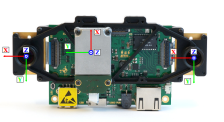
\includegraphics{images/quaternion/visensor_frames}
    \caption{VI-Sensor Coordinate Frames}
  \end{subfigure}
  ~ \quad
  \begin{subfigure}[b]{0.47\textwidth}
    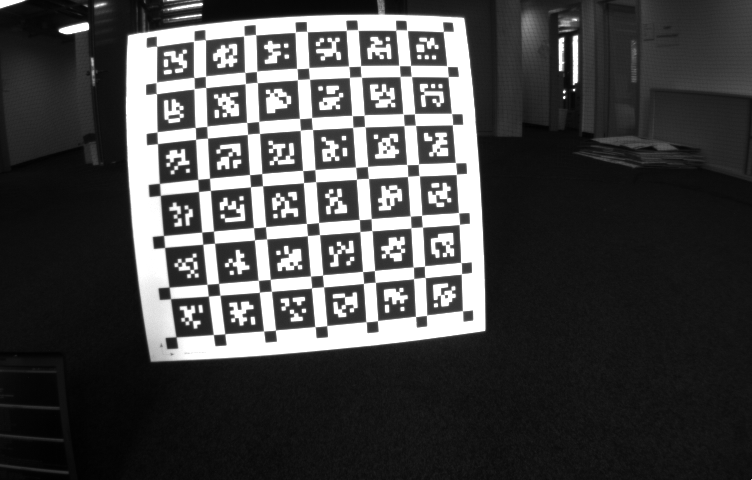
\includegraphics[width=\textwidth]{images/quaternion/1404733405732800000}
    \caption{Image frame}
  \end{subfigure}
  % \caption{EuRoC MAV Dataset - \begin{verbatim}imu_april\end{verbatim} sequence}
  \caption{EuRoC MAV Dataset - \texttt{imu\_april} Sequence}
\end{figure}

Before calculating the axis-angle, however, it should be noted that when an
accelerometer is at rest the measurement reading in the z-axis is positive
instead of negative. The reason is accelerometers measures acceleration by
measuring the displacement of a proof mass that is suspended with springs. For
example, if gravity is ignored and the accelerometer moves upwards, the proof mass
will be displaced towards the bottom of the accelerometer. This is interpreted
as an acceleration in the upwards direction, and so when the accelerometer is
at rest on a flat surface, gravity pulls on the proof mass yeilding a positive
measurement in the upwards direction. To resolve this issue the gravity vector
is negated, and so $\Vec{u} = -\Vec{g}$ and $\Vec{v} = \Vec{a}_{m}$. Using 
\eqref{eq:angle_axis_calc_angle} and \eqref{eq:angle_axis_calc_axis} the
axis-angle, $\boldsymbol{\theta}$, is thereby
%
\begin{align}
  % -- Axis-Angle
  \theta &= 1.8982 \\
  \Vec{e} &= \Transpose{
    \begin{bmatrix}
      0.03352 &
      0.99944 &
      0.00000
    \end{bmatrix}
  }
\end{align}
%
Finally the quaternion, $\quat_{\world\sensor}$, can be calculated using
\eqref{eq:quaternion_from_axis_angles} resulting in
%
\begin{equation}
  % -- Quaternion
  \quat_{\world\sensor} &= \Transpose{
    \begin{bmatrix}
      0.58240 &
      0.02725 &
      0.81245 &
      0.00000
    \end{bmatrix}
  } \enspace .
\end{equation}



% -- QUATERNION TO ROTATION MATRIX
\subsection{Quaternion to Rotation Matrix}

\begin{equation}
  \Mat{R}\{\quat \} = \begin{bmatrix}
    q_w^2 + q_x^2 - q_y^2 - q_z^2
    & 2(q_x q_y - q_w q_z)
    & 2(q_x q_z + q_w q_y) \\
    2(q_x q_y + q_w q_z)
    & q_w^2 - q_x^2 + q_y^2 - q_z^2
    & 2(q_y q_z - q_w q_x) \\
    2(q_x q_y - q_w q_y)
    & 2(q_y q_z + q_w q_x)
    & q_w^2 - q_x^2 - q_y^2 + q_z^2
  \end{bmatrix}
\end{equation}

